%
% File: chap01.tex
% Author: Victor F. Brena-Medina
% Description: Introduction chapter where the biology goes.
%
\let\textcircled=\pgftextcircled
\chapter{Designing the Switch Matrix}
\label{chap:SWITCH_MATRIX_design}
\paragraph{}

\section{Overview}

\paragraph{}
In the previous chapter, the CLB was designed based on theoretical derivations regarding area and delay. This chapter will focus on architecting and designng the Switch Matrix that will provide routability on the FPGA fabric.

\section{Switch Matrix type}
\paragraph{}

A lot of switch matrices have been proposed[8] in the academia till now including the universal switch matrix, wilton switch matrix[9] and disjoint switch matrix.
\begin{figure}[H]
\centering
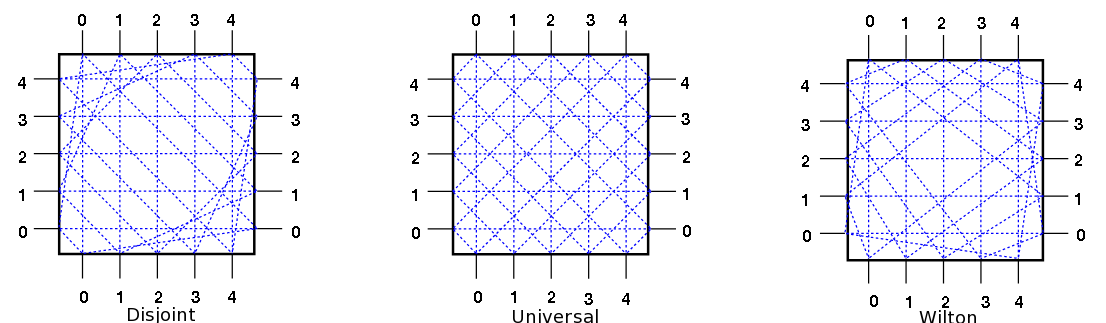
\includegraphics[width=0.9\textwidth]{switchmatrix_types.png}
\caption{Different types of switch matrices}
\label{fig:Figure}
\end{figure}
\begin{itemize}
  \item \textbf{Universal : } Universal switch matrix proposed by Chang et.al in [CWW96a, CWW96b] uses 6W switches and any two nets can be connected to each other provided that each side has less than W signals. This method is superior in routing performance but lags behind other designs in terms of area and delay.

  \item \textbf{Wilton : } Wilton switch matrix proposed by Wilton[Wil97] solves one key problem of most other SM designs. Most designs try to restrict a signal in a particular track and thus perform poorly with sparse connected designs of memories. This is because memories use pins connected on specific tracks only. Wilton proposed a solution which arbitrated the track of a signal after every SM it encountered. This makes sure that all the tracks are used evenly and thus congestion is relieved.
\begin{figure}[H]
\centering
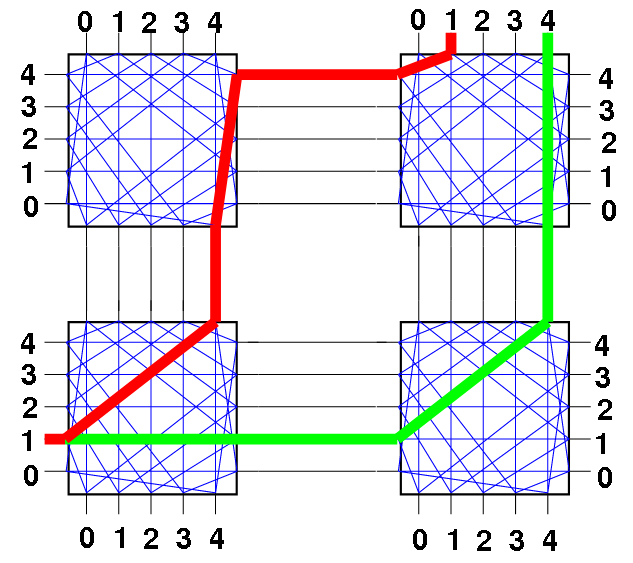
\includegraphics[width=0.4\textwidth]{wilton_possibility.png}
\caption{Routing possibilities with Wilton design}
\label{fig:Figure}
\end{figure}

  \item \textbf{Disjoint : } Disjoint switch matrix was first proposed and used by Xilinx. The design can connect a net to 4 different possibilities, one on each side. This block also suffers from the same problem of using the same track throughout leading to congestion in many areas.
\begin{figure}[H]
\centering
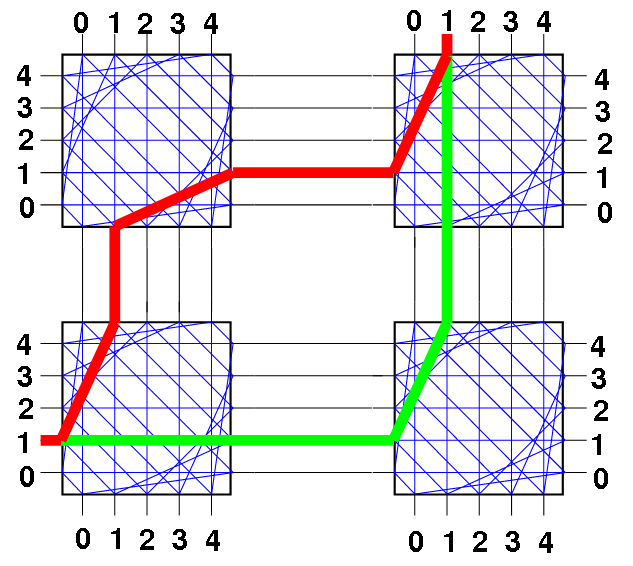
\includegraphics[width=0.4\textwidth]{disjoint_possibility.png}
\caption{Routing possibilities with Disjoint design}
\label{fig:Figure}
\end{figure}
\end{itemize} 

Due to its versatility and robustness, we stick with Wilton switch matrix design for our design and analysis purposes.

\section{Describing the FPGA in VTR}
\paragraph{}
To study the effects of connectivity fractions, orientation of input pins and output pins, routing width etc., we used VTR[4] tool. Verilog to Routing needs the architecture of the FPGA to be described in an XML format with specifications given in the relevant tags. We described our architecture in the prescribed format and kept the grid size as variable depending on the design to be implemented. We settled with MUX based one way tracks in our switch matrices to save routing area as our FPGA is only designed for minimal applications.


\section{Deciding CLB pinout}
\paragraph{}

The 4 inputs of the CLB can be taken from any of the neighbouring routing wires of the CLB. There are 2 cases to put the pins as discussed below:

\begin{itemize}
\item \textbf{All inputs of left :} This design (Fig. 4.4) will connect the input crossbar to the 4 wires passing from the left side of the CLB. This method forces all 4 signal to be brought to the left 4 wires before they can be used to perform boolean functions. This takes up all the 4 wires on a CLB's left. So the signal going from top to bottom are hindered and thus have to travel some extra distance horizontally. This phenomenon accumulates congestion quickly and thus needs larger routing widths(W) to route any given design. This can be seen in the implementation of a 5-bit adder on our FPGA (see Fig. 4.5 and 4.6).

\begin{figure}[H]
\centering
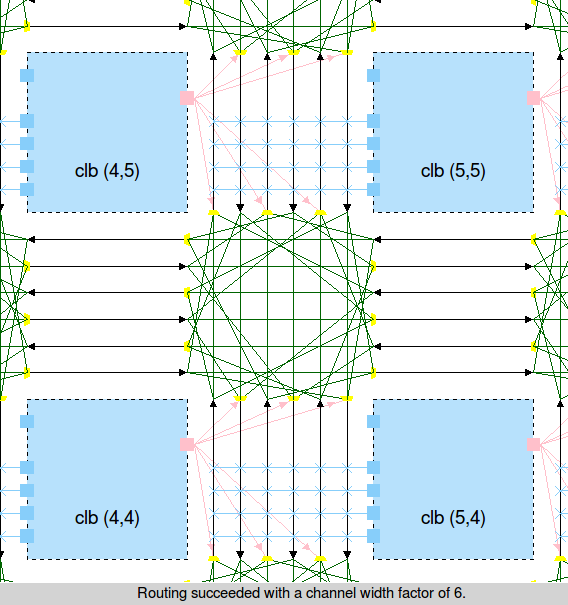
\includegraphics[scale=0.4]{BTP_work/5-bit_adder_on_left_only_clb/clb_pinout.png}
\caption{CLB pinout: all inputs on left side}
\label{fig:Figure}
\end{figure}
\begin{figure}[H]
\centering
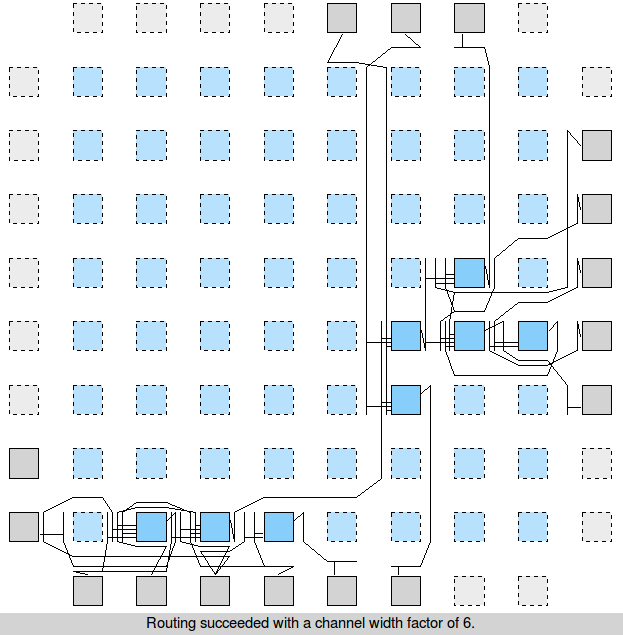
\includegraphics[scale=0.3]{BTP_work/5-bit_adder_on_left_only_clb/routing.png}
\caption{Routing of a 5-bit adder needs W=6}
\label{fig:Figure}
\end{figure}
\begin{figure}[H]
\centering
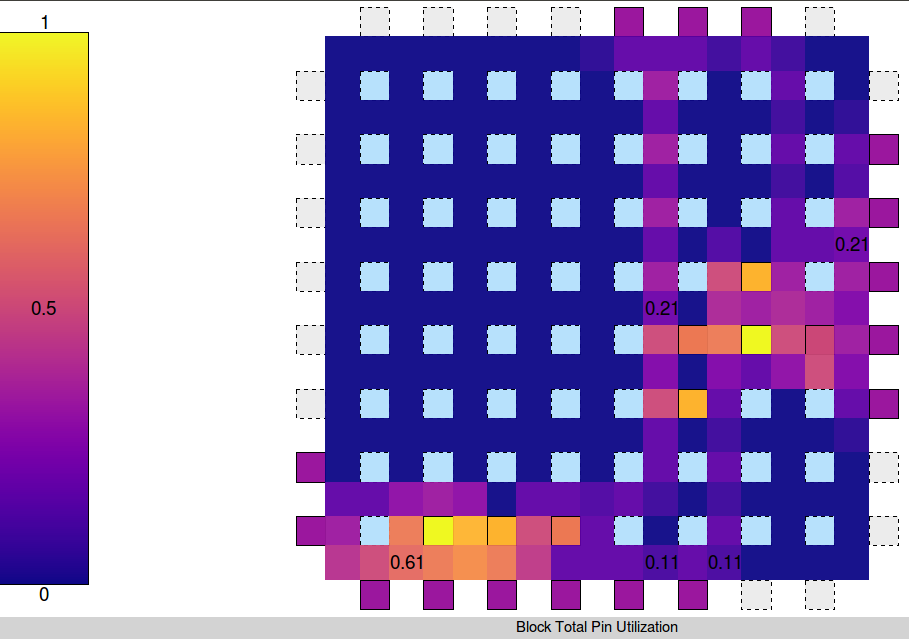
\includegraphics[scale=0.3]{BTP_work/5-bit_adder_on_left_only_clb/routing_congestion.png}
\caption{Routing congestion : all left IO}
\label{fig:Figure}
\end{figure}

\item \textbf{One input from each side :} In this design (see Fig. 4.7), the input crossbar will select one input from the left 4 wires, 1 input from the right 4 wires, 1 input from the top 4 wires and 1 input from the bottom 4 wires. Thus, all the inputs are not needed to be brough to one side of the CLB. This releives congestion and therefore can route a given logic circuit with a smaller routing width(W). This can be seen in the implementation of a 5-bit adder on our FPGA (see Fig. 4.8 and 4.9).

\begin{figure}[H]
\centering
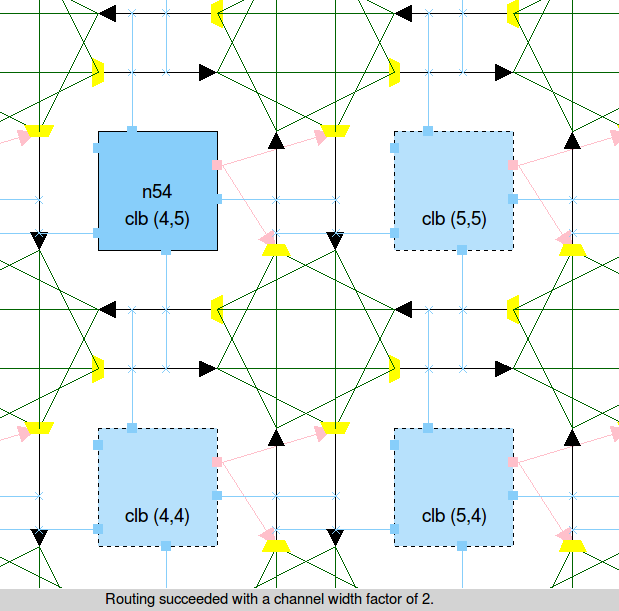
\includegraphics[scale=0.4]{BTP_work/5-bit_adder_on_spread_IO_clb/clb_pinout.png}
\caption{CLB pinout: one input from each side}
\label{fig:Figure}
\end{figure}
\begin{figure}[H]
\centering
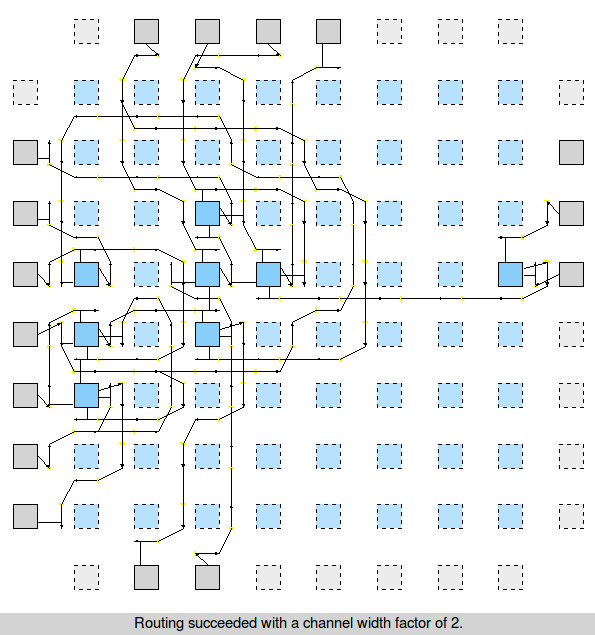
\includegraphics[scale=0.32]{BTP_work/5-bit_adder_on_spread_IO_clb/routing.png}
\caption{Routing of a 5-bit adder needs W=2}
\label{fig:Figure}
\end{figure}
\begin{figure}[H]
\centering
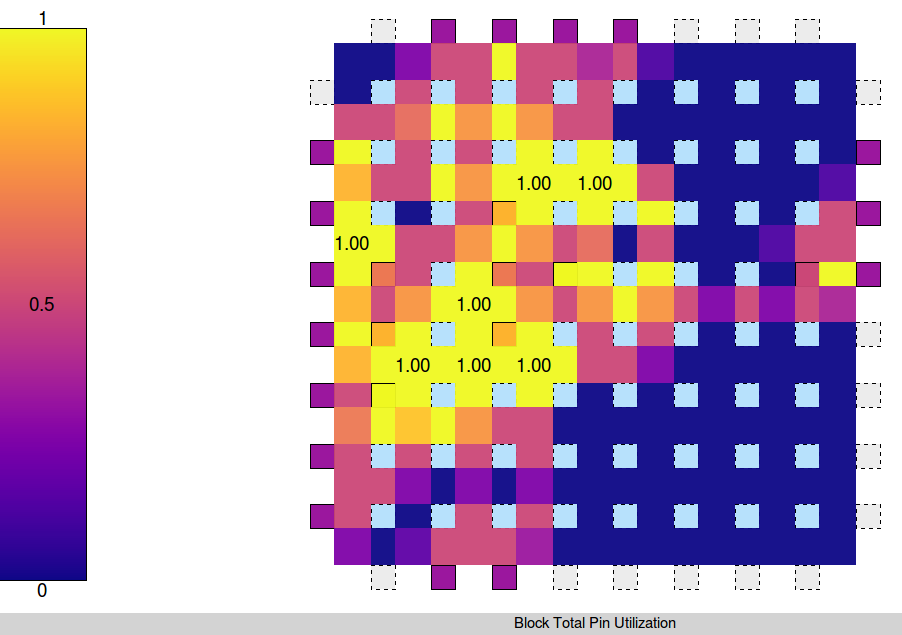
\includegraphics[scale=0.32]{BTP_work/5-bit_adder_on_spread_IO_clb/routing_congestion.png}
\caption{Routing congestion: spread IO}
\label{fig:Figure}
\end{figure}

\end{itemize}
This case study leads to the observation that taking one input from each side instead of taking all inputs from one side provides significant reductions in the routing width requirements(a factor of 3x). Thus, the area overheads in making an all sided input crossbar are easily shadowed by the area and delay benefits gained from reduction in routing width(W). Due to this, we use one input from each side for our FPGA design. 

\section{Deciding channel width}
\paragraph{}
To decide upon a channel width, we conduct experiments using vtr with various verilog designs and see how much grid size and routing width is sufficient to route these designs. Two representative verilog codes are detailed below:

\begin{itemize}

\item \textbf{10-bit adder :} This is a simple 10-bit adder which adds two given inputs to produce the sum. We find that a grid size of 8x8 and channel width of 4 are sufficient to route the design (see Fig. 4.11). We also show the routing congestion for our routed design (see Fig. 4.12).

\begin{figure}[H]
\centering
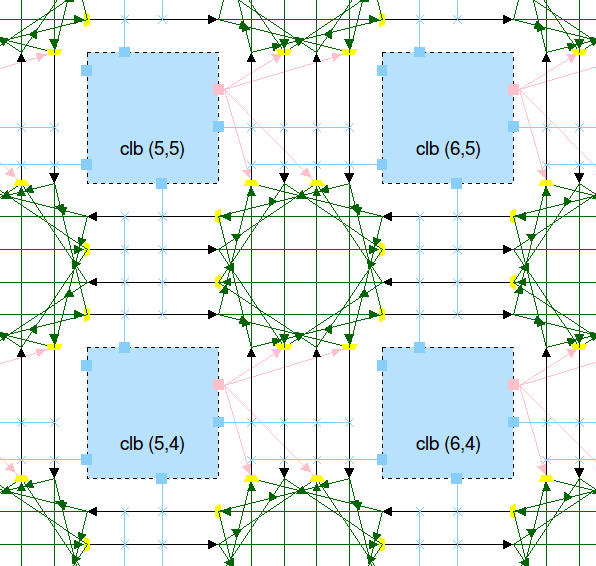
\includegraphics[scale=0.4]{BTP_work/8x8_closeup.png}
\caption{CLB pinout and switch matrix closeup}
\label{fig:Figure}
\end{figure}
\begin{figure}[H]
\centering
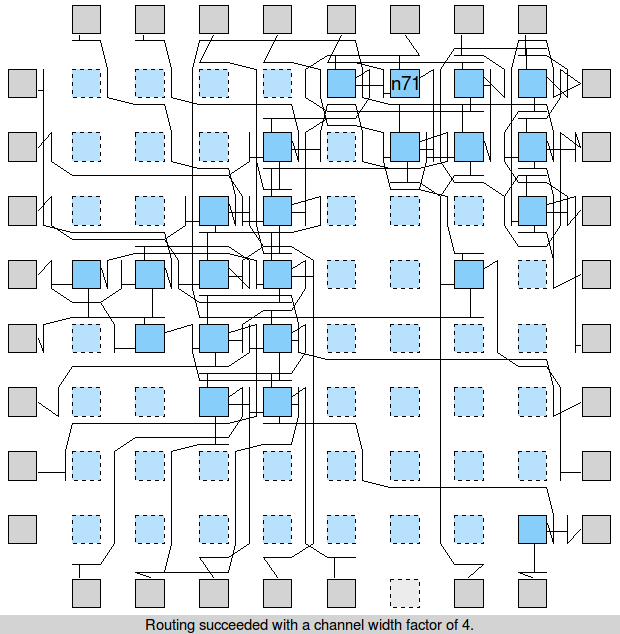
\includegraphics[scale=0.3]{BTP_work/8x8_adder_routing.png}
\caption{Routing of a 10-bit adder needs W=4}
\label{fig:Figure}
\end{figure}
\begin{figure}[H]
\centering
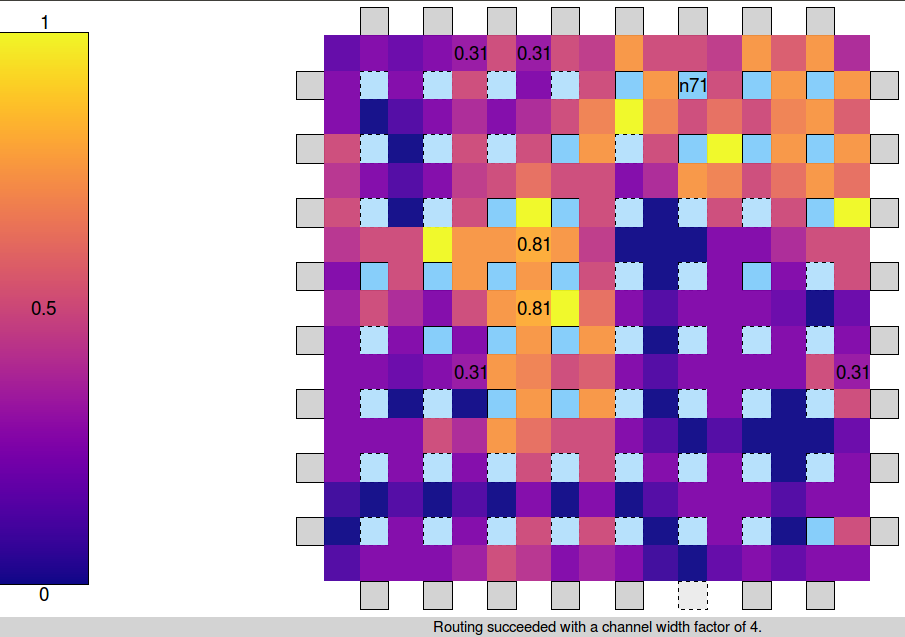
\includegraphics[scale=0.3]{BTP_work/8x8_adder_congestion.png}
\caption{Routing congestion}
\label{fig:Figure}
\end{figure}

\item \textbf{A complex memory controller :} We implement the verilog code of a complex memory controller written in Verilog on the  FPGA and find out that a grid size of 60x60 is required along with a routing width of 4 (see Fig. 4.13). We also show the routing congestion for our routed design in Fig. 4.14.

\begin{figure}[H]
\centering
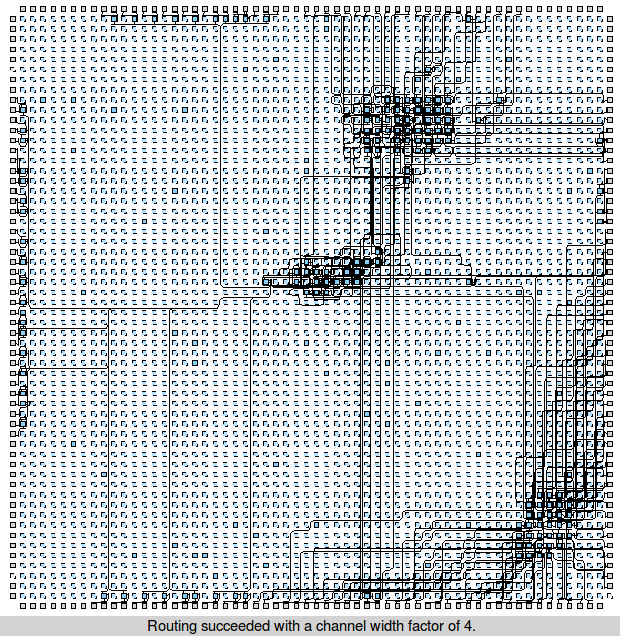
\includegraphics[scale=0.4]{BTP_work/60x60_controller_routing.png}
\caption{Routing the memory controller needs W=4}
\label{fig:Figure}
\end{figure}
\begin{figure}[H]
\centering
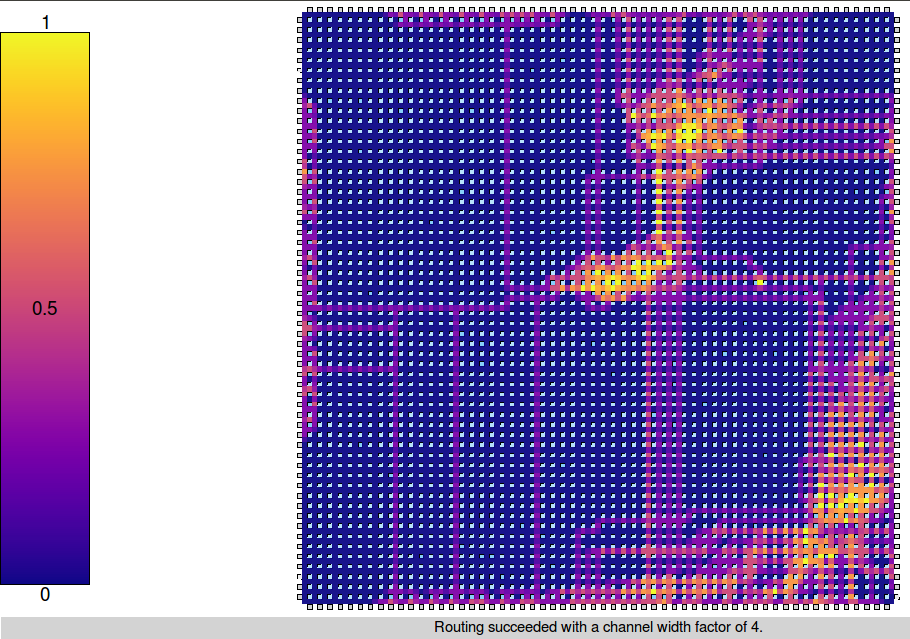
\includegraphics[scale=0.32]{BTP_work/60x60_controller_congestion.png}
\caption{Routing congestion}
\label{fig:Figure}
\end{figure}

\end{itemize}
The rest of the experiment results are summarized in Fig. 4.15:
\begin{figure}[H]
\centering
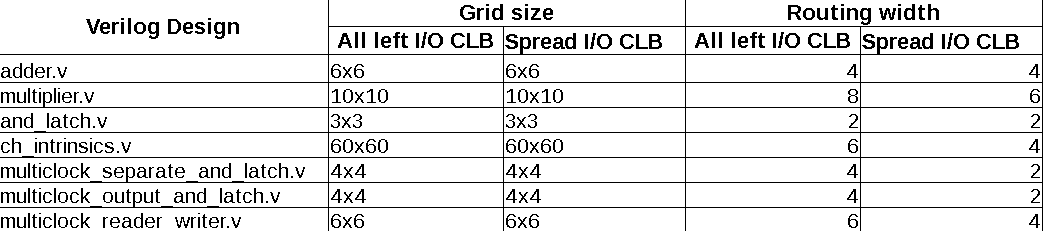
\includegraphics[scale=0.42]{analysis_table.png}
\caption{Required grid sizes and routing widths for different verilog designs}
\label{fig:Figure}
\end{figure}
From this table, we observe that the grid size scales with complex logic circuits but the channel width of 4 is still sufficient for most of the designs we used. This dictates our choice of a channel width factor of 4 for our FPGA design so that we can scale the FPGA if needed without changing the routing.

\section{Summary}
\paragraph{}
This chapter describes the architecture choices that went into deciding on the structure of the switch matrix. Since we use MUX based switch matrices of width 4, 16 bits are required for configuring each switch matrix. These 16 bits are organized as a 4*4 SRAM array. The switch matrix is simulated for functional correctness in ADE L using spectre. The schematic described in Cadence schematic and the waveforms are presented in Fig. 4.16 and 4.17 respectively.

\begin{figure}[H]
\centering
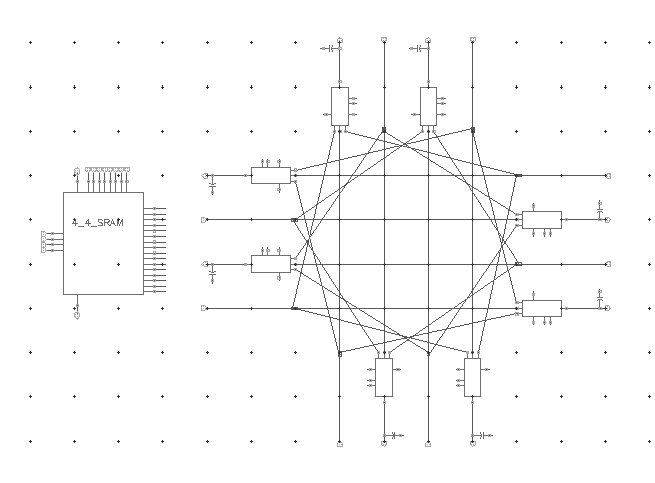
\includegraphics[scale=0.58]{sm.png}
\caption{Schematic of Switch Matrix}
\label{fig:Figure}
\end{figure}
\begin{figure}[H]
\centering
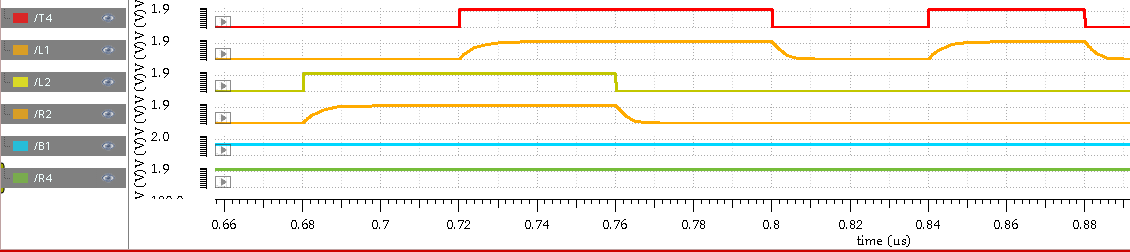
\includegraphics[width=\textwidth]{smsimulation.png}
\caption{Simulation results of Switch Matrix - Center}
\label{fig:Figure}
\end{figure}

The final FPGA architecture described in VTR is presented in Fig. 4.18.

\begin{figure}[H]
\centering
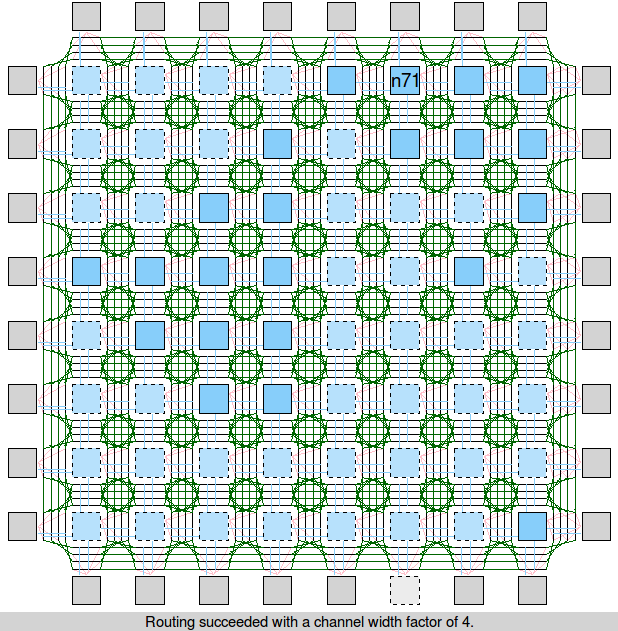
\includegraphics[scale=0.65]{BTP_work/8x8_FPGA.png}
\caption{8x8 FPGA structure as seen in VTR}
\label{fig:Figure}
\end{figure}


